\documentclass[../main.tex]{subfiles}
\usepackage{float}

\begin{document}


%tabla 1
%tabla 2

Para identificar notoriamente el desplazamiento del resorte en dirección vertical, se combinaron masas con la siguiente configuración:

%tabla 3

Para determinar el valor de la constante K de los resortes, es preciso considerar la
fuerza neta que actúan sobre ellos, en este caso, la fuerza de la gravedad o peso.
Para este informe, se tomará el valor de la gravedad redondeado a 4 cifras 
significativas $\ (9,807 \, m/s^2\ )$. Asimismo, se trabajará con el SI
de unidades, haciendo la conversión de centímetros a metros. Por otro lado, se determinará 
la constante K para cada elongación, de esta manera, empleando el método de la 
desviación estándar se calculará su incertidumbre según sea el caso.
Se sabe por la ecuación () que $ K = Peso \cdot \Delta L$, entonces:

%tabla 4

Un detalle a considerar es que en la tabla 4, los valores de K para ambos resortes 
según cada elongación, no fueron redondeados siguiendo las reglas de cifras significativas, con el propósito de obtener un cálculo más preciso de la desviación estándar, de hecho, se consideró 4 cifras significativas.

%grafica 1
\begin{figure}[H]
    \centering
    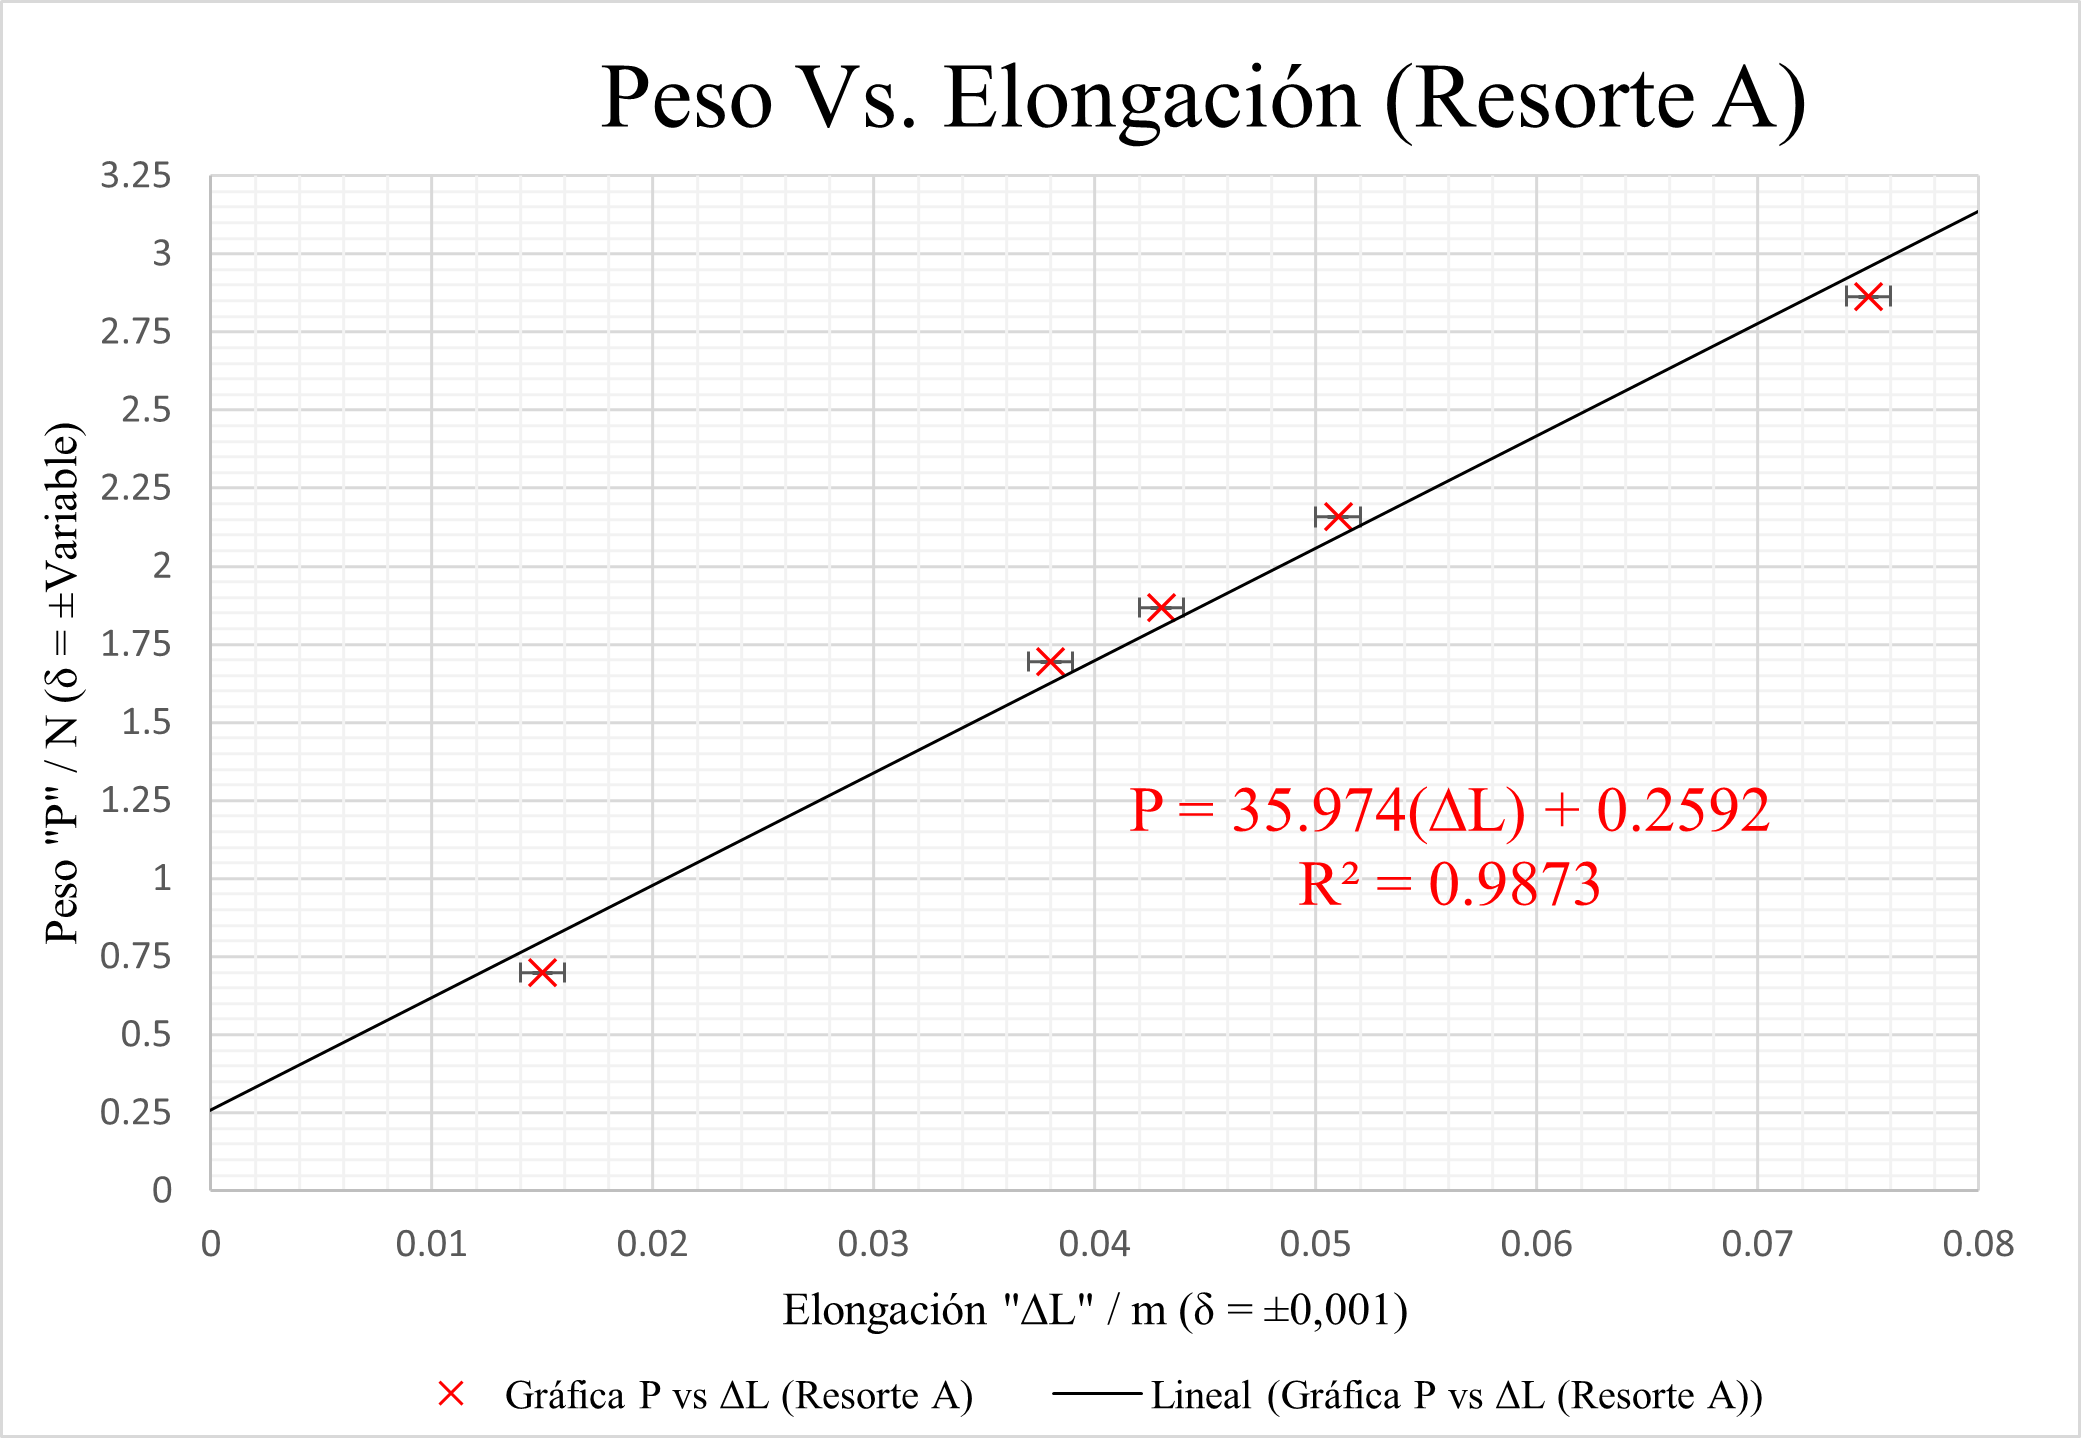
\includegraphics[width=0.8\linewidth]{images/calc1.png}
    \label{ref:calc1}
    \caption{Peso en función de la elongación del resorte A.}
\end{figure}
%grafica 2
\begin{figure}[H]
    \centering
    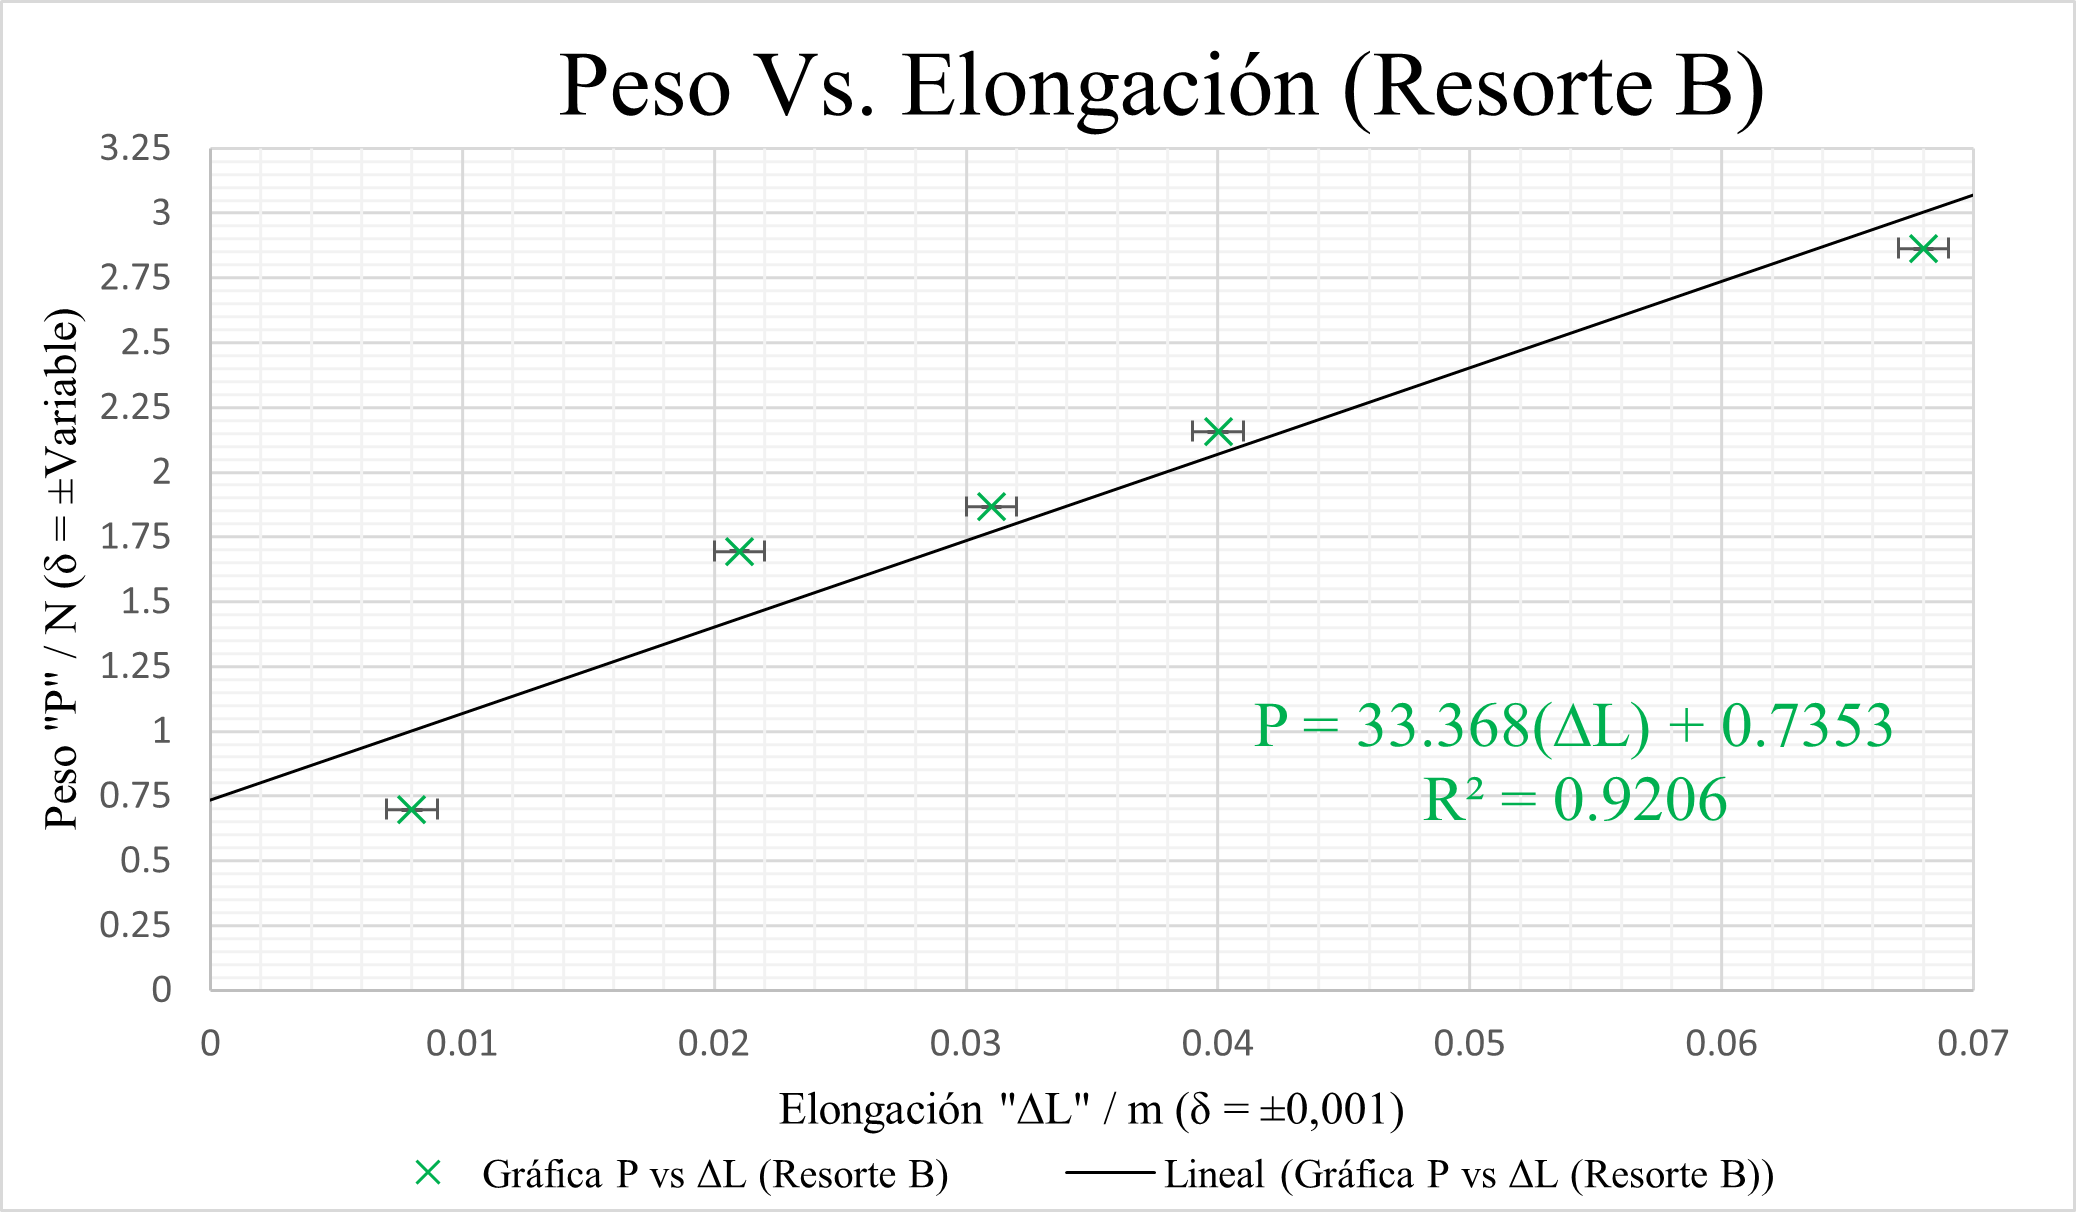
\includegraphics[width=0.8\linewidth]{images/calc2.png}
    \label{ref:calc2}
    \caption{Peso en función de la elongación del resorte B.}
\end{figure}

Mediante las gráficas 1 y 2 de tendencia lineal se puede determinar la
constante K de cada resorte, para ello, se evaluarán sus respectivas ecuaciones:
Resorte A:

\[P=35,974 \Delta  L +0,2592…()\]

La pendiente de la ecuación () es 35,974; y 36 según redondeo a cifras significativas. 
Por otro lado, tratándose de un ajuste lineal basado en datos experimentales, la ecuación () 
posee un término independiente que no concuerda con la ecuación lineal de la ley de
Hooke, por lo cual, se asumirá irrelevante este valor respecto al valor de la pendiente.\\
Entonces:
\[P = K \cdot \Delta L = 36 \cdot (\Delta L) \]
\[K_A=36\ N/m\]
Se verifica que la pendiente es en realidad la constante del resorte A, denotada como 
$K_A$.
Para determinar la incertidumbre, se calculará la desviación estándar (ecuación ()) de los
datos obtenidos de las constantes del resorte de los datos experimentales.
\[\Delta K_A\ =\ \sum_{i\ =\ 1}^{5}\frac{{(k_{i\ }\ -\ \bar{k})}^2}{10}\ =2,792\frac{N}{m}\approx3\ N/m\]
La medida de la constante del resorte A es: $K_A \pm \Delta K_A=(36\pm 3)\ N/m$\\
Ahora mediante el método del error relativo, se evaluará la precisión del resultado comparándolo con su incertidumbre:
\[\varepsilon_{RK_A} = \frac{3}{36} = 0,08 \approx 8\%\]
Como se observa, la medida está dentro del rango de lo aceptable en cuanto a precisión, 
es decir, menor a 10 \% de error relativo.\\
Respecto a la fiabilidad del ajuste lineal, el coeficiente de determinación (R2) muy 
cercano a la unidad indica que ambas rectas se adaptan casi al 100\% a la tendencia
de los datos experimentales.\\
Resorte B:
\[P=33,368 \Delta L+0,7353…()\]
La pendiente de la ecuación () es 33,368; y 33 según redondeo a cifras significativas. \\
Del mismo modo que en el resorte A, el término independiente se descarta de la 
ecuación, esto, por un lado, induce al error, considerando, además, que el término
independiente de la ecuación () es mayor que el de la ecuación (),
pero la ventaja es que permite establecer una correlación directa con la fórmula teórica.

\[P=K \Delta L=33 \Delta L\]
\[K_B=33\ N/m\]
Se verifica que la pendiente es en realidad la constante del resorte 2, denotada como K2.
Empleando la ecuación de la desviación estándar para hallar la incertidumbre.

\[\Delta K_B\ =\ \sum_{i\ =\ 1}^{5}\frac{{(k_{i\ }\ -\ \bar{k})}^2}{10}\ =16,80\frac{N}{m}\approx 17 \, N/m\]

La medida de la constante del resorte B es: $K_B \pm \Delta K_B=(33 \pm 17) \, N/m$ \\

Ahora mediante el método del error relativo, se evaluará la precisión del resultado comparándolo con su incertidumbre:

\[\varepsilon_{RK_B}=\frac{17}{33}=0,52\approx52\%\]

Como se logra apreciar, el error relativo es 5 veces mayor a 10\%,
lo cual indica que la precisión es bastante baja en comparación con la
medida del resorte A, esto podría deberse a una mala medición de la elongación
del resorte, probablemente una sola medida que provocó que la constante del 
resorte para ese dato fuese un valor muy alejado de los demás, también se observa
en la tabla 4, que la constante ki del resorte B tiende a disminuir a medida que 
el peso aumenta, dando a entender que la medición se hace más sensible mientras mayor 
sean las magnitudes del peso y la elongación. Otra posible causa, es la forma del resorte,
puesto que, al realizar la medición en el laboratorio, este tenía una cierta deformación 
en dirección horizontal, lo cual pudo afectar la toma de datos significativamente.

%tabla 5

Donde $\vec{r}_A$ y $\vec{r}_B$ representan el vector posición medido desde A y B
respectivamente, hasta los puntos (ticks) señalados de la trayectoria curvilínea en
forma de “e”.

%tabla 6

Cabe resaltar que los ángulos señalados en la tabla 6, fueron medidos en posición normal.

\textbf{Cálculo de la fuerza resultannte en los puntos 7; 13 Y 18 ticks}

Para hallar la fuerza resultante ejercida por los resortes A y B en los puntos 7; 13 y 18, 
se procedió a descomponer vectorialmente las fuerzas $\vec{A}$ y $\vec{B}$ en función 
al ángulo que formaba con la horizontal como lo muestra la tabla 6.

\[\sum{\vec{F}}= \vec{F_A} + \vec{F_B}\]
\[\vec{F_A}+\vec{F_B}=\ (F_{Ax}+F_{Ay}\ )+\ (F_{Bx}+F_{By}\ )\]
\[\vec{F_A}+\vec{F_B}=F_A\ (\cos{\alpha}\ \hat{i}+sen\ \alpha\ \hat{j}\ )+F_B\ (\cos{\beta}\ \hat{i}+sen\ \beta\ \hat{j}\ )\]
\[\vec{F_A}+\vec{F_B}=\vec{F_R}\]

Donde $\alpha$ y $\beta$ son los ángulos que forman las fuerzas $\vec{A}$ y $\vec{B}$ 
respectivamente con el eje de las abscisas, y $\vec{F_R}$ el vector fuerza resultante.\\

No obstante, cómo determinar el módulo de las fuerzas $\vec{A}$ y $\vec{B}$ si no se puede hacer 
uso de la segunda ley de Newton, pues se desea comprobar la validación de esta teoría. La mejor
forma es empleando la ley de Hooke descrita previamente en la base teórica.

\[\vec{F}=\vec{r} \cdot K\]

Donde $\vec{r}$ es el desplazamiento de la masa unida al resorte, y “K” es la
constante elástica del resorte. Entonces, utilizando los datos hallados
anteriormente sobre K:

\[\vec{F_A}+\vec{F_B}=\ [\ (\ |{\vec{r}}_{At}\ |\ )\ (K_A\ )\ (\cos{\alpha}\ \hat{i}+sen\ \alpha\ \hat{j}\ )\ ]+\ [\ (\ |{\vec{r}}_{Bt}\ |\ )\ (K_B\ )\ (\cos{\beta}\ \hat{i}+sen\ \beta\ \hat{j}\ )\ ]\]

Donde $\vec{r}_{At}$ y $\vec{r}_{Bt}$ representan el módulo del desplazamiento respecto 
de A y B respectivamente, en un tick determinado.\\

\textbf{Para el instante t = 7 ticks:}

\begin{equation*}
        \vec{F_A} + \vec{F_B} = [ ( r_{A7} ) (K_A)
        (\cos{\alpha} \hat{i} + sen \, \alpha \, \hat{j} ) ] +  [ ( |
        r_{B7} ) (K_B ) (\cos{\beta} \hat{i}+sen \beta \hat{j} ) ]
    \\
    \vec{F_{R7}}=0,237036cos 6,0° i+sen 6,0° j+0,176033cos173,0° i+sen 173,0° j
    \\
    \vec{F_R}=\ (2,7\ \hat{i}+1,6\ \hat{j}\ )\ N
\end{equation*}

Módulo de la fuerza resultante para t = 7 ticks:

\begin{equation*}
    F_R = \sqrt{(2,7)^2 + (1,6)^2}
    F_R = 3,1\ N
\end{equation*}

\textbf{Para el instante t = 13 ticks:}
\[\vec{F_A}+\vec{F_B}=\ [\ (\ |{\vec{r}}_{A13}\ |\ )\ (K_A\ )\ (\cos{\alpha}\ \hat{i}+sen\ \alpha\ \hat{j}\ )\ ]+\ [\ (\ |{\vec{r}}_{B13}\ |\ )\ (K_B\ )\ (\cos{\beta}\ \hat{i}+sen\ \beta\ \hat{j}\ )\ ]\]
\[\vec{F_{R13}}=0,289036cos-29,0°i+sen-29,0° j+0,213033cos-138,0°i+sen-138,0° j\]
\[\vec{F_R}=\ (3,9\ \hat{i}-9,7\ \hat{j}\ )\ N\]
Módulo de la fuerza resultante para t = 13   ticks:
\[\ F_R = \sqrt{\ (3,9\ )^2+\ (-9,7\ )^2}\]
\[\ F_R =10 N\]


\textbf{Para el instante t = 18 ticks:}
\[\vec{F_A}+\vec{F_B}=\ [\ (\ |{\vec{r}}_{A18}\ |\ )\ 
(K_A\ )\ (\cos{\alpha}\ \hat{i}+sen\ \alpha\ \hat{j}\ )\ ]+\ [\ (\ |{\vec{r}}_{B18}\ |\ )\ (K_B\ )\ (\cos{\beta}\ \hat{i}+sen\ \beta\ \hat{j}\ )\ ]\]
\[\vec{F_{R18}}=0,146036cos-9,0° i+sen-9,0° j+0,268033cos-174,0° i+sen-174,0° j \]
\[\vec{F_R}=\ (-3,6\ \hat{i}-1,7\ \hat{j}\ )\ N\]
Módulo de la fuerza resultante para t = 18 ticks:
\[\ |\vec{F_R}\ |=\sqrt{\ (-3,6\ )^2+\ (-1,7\ )^2}\]
\[\ |\vec{F_R}\ |=4,0\ N\]

%imagen 1
\begin{figure}[H]
    \centering
    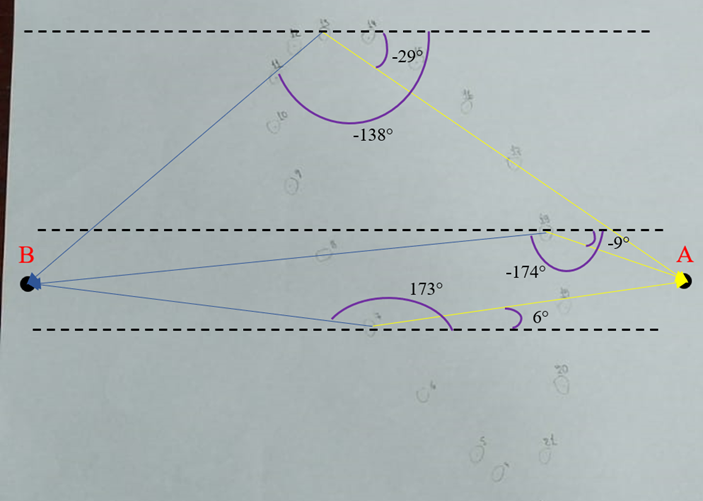
\includegraphics[width=0.8\linewidth]{images/calc3.png}
    \label{ref:calc3}
    \caption{Vectores de fuerza que ejercen $\vec{\mathbf{A}}$ y $\vec{\mathbf{B}}$ en los puntos indicados}
\end{figure}

Utilizando el método del paralelogramo, el vector fuerza resultante es: 

%imagen 2
\begin{figure}[H]
    \centering
    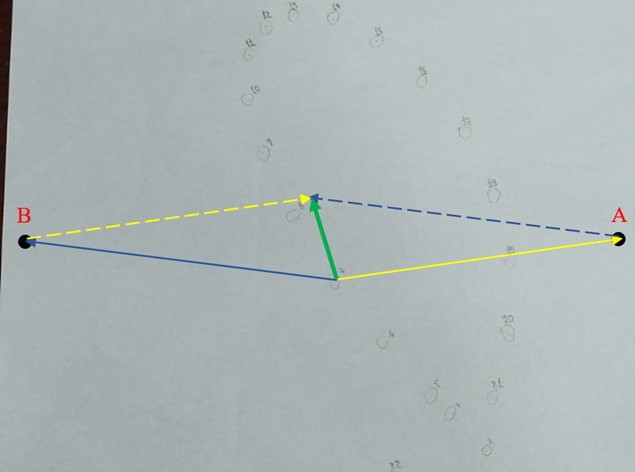
\includegraphics[width=0.8\linewidth]{images/calc4.png}
    \label{ref:calc4}
    \caption{Para el instante t = 7 ticks}
\end{figure}

%imagen 3
\begin{figure}[H]
    \centering
    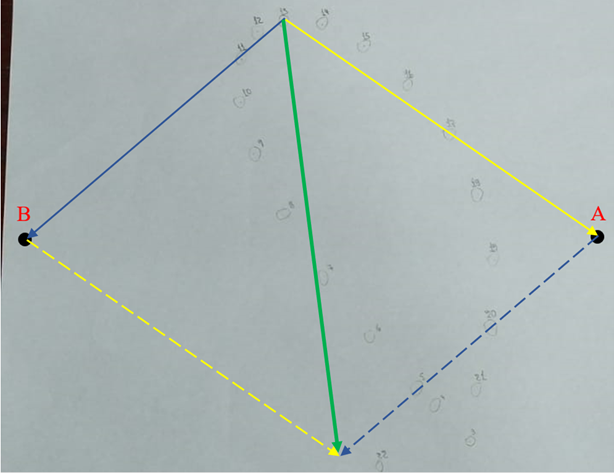
\includegraphics[width=0.8\linewidth]{images/calc5.png}
    \label{ref:calc5}
    \caption{Para el instante t = 13 ticks}
\end{figure}
%imagen 4
\begin{figure}[H]
    \centering
    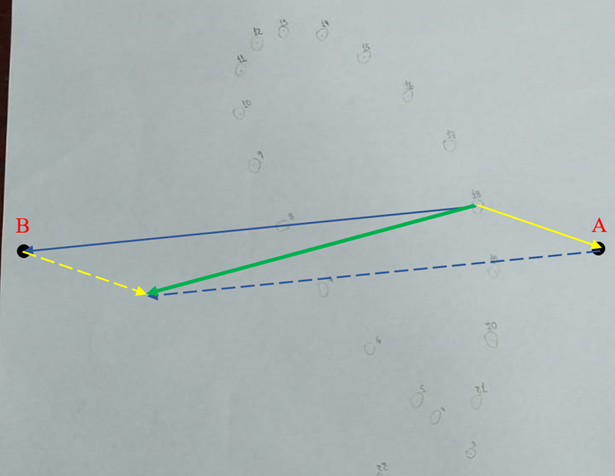
\includegraphics[width=0.8\linewidth]{images/calc6.png}
    \label{ref:calc6}
    \caption{Para el instante t = 18 ticks}
\end{figure}

\textbf{Cáculo de la aceleración instantánea en los puntos 7; 13 Y 18 ticks}
Para hallar la aceleración instantánea en los puntos seleccionados, es preciso
calcular en primer lugar, las velocidades instantáneas en puntos intermedios de
los ticks más cercanos al punto que se desea estudiar. Para ello, se tomará como 
referencia los vectores posición con un sistema de referencia fijo en B,
 por lo cual es preciso conocer los ángulos que forma cada vector con el 
 eje horizontal, de esa manera, se podrá determinar la magnitud y dirección
  de la aceleración instantánea:

%tabla 7

Los siguientes cálculos se realizarán utilizando el método de descomposición vectorial con punto de origen en B. Cabe resaltar que la frecuencia de cada tick es 20 Hz, por lo cual,
el tiempo transcurrido entre cada tick es $\frac{1}{20}$ s.

%tabla 8

Para el instante t = 7 ticks:

\[\vec{V}\left(6,5\right)=\frac{{\vec{r}}_7-{\vec{r}}_6}{1\ tick}=0,1760cos173,0°i+sen173,0° j-0,2060cos163,0°i+sen163,0° j1 tick\]

\[V\left(6,5\right)=0,02231\ \hat{i}-0,03878\ \hat{j}\ \frac{m}{tick}\]

\[\vec{V}\left(7,5\right)=\frac{{\vec{r}}_8-{\vec{r}}_7}{1\ tick}=0,1530cos-173,0°i+sen(-173,0°)j-0,1760cos173,0°i+sen173,0°j1 tick\]
\[V\left(7,5\right)=0,02283\ \hat{i}-0,04010\ \hat{j}\ \frac{m}{tick}\]

\[\vec{a}\left(7\right)=\frac{V\left(7,5\right)-V\left(6,5\right)}{1\ tick}=\ \frac{\left(0,02283\ \hat{i}-0,04010\ \hat{j}\right)-\left(0,02231\ \hat{i}-0,03878\ \hat{j}\right)}{1\ {tick}^2}\]

\[\vec{a}\left(7\right)=\frac{0,0005200\ \hat{i}-0,001320\ \hat{j}}{1\ {tick}^2}\]

\[\vec{a}\left(7\right)=400\left[\frac{0,0005200\ \hat{i}-0,001320\ \hat{j}}{1\ s^2}\right]=\ 0,208\ \hat{i}-0,528\ \hat{j}\ \frac{m}{s^2}\]


Módulo de la aceleración para t = 7 ticks:
\[a=\sqrt{\left(0,208\right)^2+\left(-0,528\right)^2}\approx0,567\ \frac{m}{s^2}\ \]

\textbf{Para el instante t = 13 ticks:}

\[\vec{V}\left(12,5\right)=\frac{{\vec{r}}_{13}-{\vec{r}}_{12}}{1\ tick}=0,2130cos-138,0°i+sen(-138,0°)j-0,1960cos-136,0°i+sen-136,0° j1 tick\]
\[V\left(12,5\right)=-0,01730\ \hat{i}-0,006372\ \hat{j}\ \frac{m}{tick}\]
\[\vec{V}\left(13,5\right)=\frac{{\vec{r}}_{14}-{\vec{r}}_{13}}{1\ tick}=0,2290cos-142,0°i+sen(-142,0°)j-0,2130cos-138,0°i+sen(-138,0°)j1 tick\]
\[V\left(13,5\right)=-0,02216\ \hat{i}+0,001538\ \hat{j}\ \frac{m}{tick}\]
\[\vec{a}\left(13\right)=\frac{V\left(13,5\right)-V\left(12,5\right)}{1\ tick}=\ \frac{\left(-0,02216\ \hat{i}+0,001538\ \hat{j}\right)-\left(-0,01730\ \hat{i}-0,006372\ \hat{j}\right)}{1\ {tick}^2}\]
\[\vec{a}\left(13\right)=\frac{-0,004860\ \hat{i}+0,007910\ \hat{j}}{1\ {tick}^2}\]\
\[\vec{a}\left(13\right)=400\left[\frac{-0,004860\ \hat{i}+0,007910\ \hat{j}}{1\ s^2}\right]=-1,94\ \hat{i}+3,16\ \hat{j}\ \frac{m}{s^2}\]

Módulo de la aceleración para t = 13 ticks:
\[\left|\vec{a}\right|=\sqrt{\left(-1,94\right)^2+\left(3,16\right)^2}\approx3,71\ \frac{m}{s^2}\]

\textbf{Para el instante t = 18 ticks:}
\[\vec{V}\left(17,5\right)=\frac{{\vec{r}}_{18}-{\vec{r}}_{17}}{1\ tick}=0,2680cos-174,0°i+sen(-174,0°)j-0,2610cos-165,0°i+sen-165,0° j1 tick\]
\[V\left(17,5\right)=-0,01443\ \hat{i}+0,03954\ \hat{j}\ \frac{m}{tick}\]
\[\vec{V}\left(18,5\right)=\frac{{\vec{r}}_{19}-{\vec{r}}_{18}}{1\ tick}=0,2730cos176,0°i+sen(176,0°)j-0,2680cos-174,0°i+sen(-174,0°)j1 tick\]
\[V\left(18,5\right)=-0,005803\ \hat{i}+0,04706\ \hat{j}\ \frac{m}{tick}\]
\[\vec{a}\left(18\right)=\frac{V\left(18,5\right)-V\left(17,5\right)}{1\ tick}=\ \frac{\left(-0,005803\ \hat{i}+0,04706\ \hat{j}\right)-\left(-0,01443\ \hat{i}+0,03954\ \hat{j}\right)}{1\ {tick}^2}\]

\[\vec{a}\left(18\right)=\frac{0,008627\ \hat{i}+0,00752\ \hat{j}}{1\ {tick}^2}\]

\[\vec{a}\left(18\right)=400\left[\frac{0,008627\ \hat{i}+0,00752\ \hat{j}}{1\ s^2}\right]=3,45\ \hat{i}+3,01\ \hat{j}\ \frac{m}{s^2}\]

Módulo de la aceleración para t = 18 ticks:

\[\left|\vec{a}\right|=\sqrt{\left(3,45\right)^2+\left(3,01\right)^2}\approx4,58\ \frac{m}{s^2}\ \]

Luego para hallar el ángulo que forman los vectores fuerza y la aceleración en cada punto, se empleó la siguiente ecuación:
\[ \cos{\beta}=\frac{\vec{F}\bullet\vec{a}}{\left|\vec{F}\right|\left|\vec{a}\right|} \]
\[ \beta=\cos^{-1}{\left(\frac{\vec{F}\bullet\vec{a}}{\left|\vec{F}\right|\left|\vec{a}\right|}\right)} \]

Donde $\beta$ representa el ángulo entre los vectores fuerza y aceleración, $\vec{F}$ y $\vec{a}$ los vectores
fuerza y aceleración respectivamente, mientras que $\left|\vec{F}\right|$ y $\left|\vec{a}\right|$ simbolizan 
sus módulos. Por tanto:

\textbf{Para el instante t = 7 ticks:}
\[\beta=\cos^{-1}{\left[\frac{\left(2,7\ \hat{i}+1,6\ \hat{j}\right)\bullet\left(0,208\ \hat{i}-0,528\ \hat{j}\ \right)}{\left(3,1\right)\left(0,567\right)}\right]}\]
\[\beta=\cos^{-1}{\left[\frac{\left(2,7\right)\left(0,208\right)+\left(1,6\right)\left(-0,528\right)}{\left(3,1\right)\left(8,50\right)}\right]}\]

\[\beta\approx91°\]
\textbf{Para el instante t = 13 ticks:}
\[\beta=\cos^{-1}{\left[\frac{\left(3,9\ \hat{i}-9,7\ \hat{j}\right)\bullet\left(-1,94\ \hat{i}+3,16\ \hat{j}\right)}{\left(10\right)\left(3,71\right)}\right]}\]
\[\beta=\cos^{-1}{\left[\frac{\left(3,9\right)\left(-1,94\right)+\left(-9,7\right)\left(3,16\right)}{\left(10\right)\left(3,71\right)}\right]}\]
\[\beta=\cos^{-1}{\left[-1,03\right]}\]
En este caso el valor dentro del arco coseno es menor que -1, pero muy próximo al mismo, por tanto:
\[\beta\approx180°\]
\textbf{Para el instante t = 18 ticks:}
\[\beta=\cos^{-1}{\left[\frac{\left(-3,6\ \hat{i}-1,7\ \hat{j}\right)\bullet\left(3,45\ \hat{i}+3,01\ \hat{j}\right)}{\left(4,0\right)\left(4,58\right)}\right]}\]
\[\beta=\cos^{-1}{\left[\frac{\left(-3,6\right)\left(3,45\right)+\left(-1,7\right)\left(3,01\right)}{\left(4,0\right)\left(4,58\right)}\right]}\]
\[\beta\approx163°\]

%tabla 9

%imagen 5
\begin{figure}[H]
    \centering
    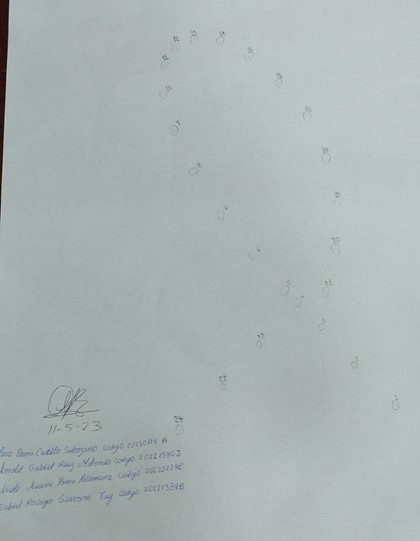
\includegraphics[width=0.8\linewidth]{images/calc7.jpg}
    \label{ref:calc7}
    \caption{Trayectoria curva en forma de “e” descrita por los puntos generados por el chispero electrónico.}
\end{figure}



\end{document}